\documentclass[border=4pt]{standalone}
\usepackage{tikz}
\usetikzlibrary{decorations.pathmorphing,arrows.meta}
\begin{document}
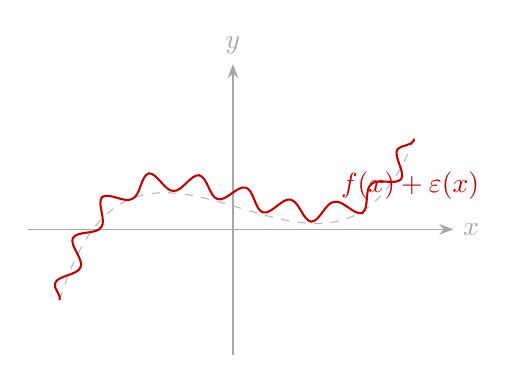
\begin{tikzpicture}
  \draw[-{Stealth[length=1.8mm]},gray!70] (-2.6,0) -- (2.8,0) node[right] {$x$};
  \draw[-{Stealth[length=1.8mm]},gray!70] (0,-1.6) -- (0,2.1) node[above] {$y$};
  \draw[gray!55,dashed] (-2.2,-.9) .. controls (-1.2,2.4) and (1.2,-1.7) .. (2.3,1.15);
  \draw[red!75!black,line width=.75pt,decorate,
    decoration={snake,segment length=6mm,amplitude=1.2mm}]
    (-2.2,-.9) .. controls (-1.2,2.4) and (1.2,-1.7) .. (2.3,1.15);
  \node[red!75!black,above right] at (1.25,.25) {$f(x)+\varepsilon(x)$};
\end{tikzpicture}
\end{document}
